%%
% 下のコメント欄は卒論執筆時の森がイキって書いたものです。
% 修論執筆時の森が代わりに謝罪いたします。
% 温かい目で見守ってあげてください。
%
% また、修論執筆時にはTeXstudioで、またDockerを用いて執筆しています。
% 上記の手法は平木場くんから教えていただきました。
% 参考: https://qiita.com/Shitimi_613/items/9706d57fb7bc17cbed0e
%

%%
% モダンなLaTeXを書きたい?
% そしたら僕の考えた最強のtexファイルを見てくれ
%
% 注意!
% このLaTeXをPDFに変換するためには、普通とはちょっと違う方法を使うよ
% コマンド上では
%   $ ptex2pdf -u -l GraduatePaper.tex
% で変換してね
% もしptex2pdfコマンドが無かったら、
%   $ uplatex GraduatePaper.tex
%   $ dvipdfmx GraduatePaper.dvi
% でうまくいくかも(未確認)
%
% え、TeXworksで使いたいって?
% そしたら、TeXworksの編集メニュー -> 設定を開く
% タイプセットタブの下の方にあるタイプセットの方法の右下の+ボタンを選択する
% 名前: uplatex(ptex2pdf)
% プログラム: ptex2pdf
% 引数: -l
%       -u
%       -ot
%       $synctexoption
%       $fullname
% として保存して、TeXworks実行ボタン右のコンボボックスのuplatex(ptex2pdf)を選択して変換だ!
%


%%
% 今時jarticleやjbook使ってる人いる?時代はjsarticleかjsbookだよ
% ついでに言うと、uplatexってのはplatexの上位互換、これを使わないなんて旧世代だよね
%
\documentclass[uplatex, report, a4j, 10pt]{jsbook}


%%
% パッケージ群
%
\usepackage{packages/miyazaki-u-paper}   % 宮崎大学工学部の卒論の基本(片山先生作)を、僕がちょっと書き換えちゃった(テヘッ
\usepackage{enumitem}           % enumerate?古い古い
\usepackage[dvipdfmx]{graphicx} % 当然dvipdfmなんて使ってないよね
\usepackage[dvipdfmx]{color}    % listingsを使うときにはこれも必須、dvipdfmxを変えちゃうとgraphicxのdvipdfmxも変わるよ
\usepackage{listings, packages/jlisting} % コードを埋め込むなら必須
\usepackage{txfonts}            % フォントといえばやっぱりtxfonts、今はnewtxってのもあるらしい
\usepackage{verbatim}           % コメントアウトしてくれる便利なプリアンブルが使える \begin{comment} ... \end{comment}
\usepackage[hdivide={21mm, , 21mm}, vdivide={30mm, , 25mm}]{geometry} % スタイルを少し変えたくても\hoffset, \voffsetは使わないでね
%\RequirePackage[l2tabu, orthodox]{nag} % これを入れると、古いコマンドを警告してくれる!なお完全には消せなかった模様

%%
% マクロの定義
%
\newcommand{\tool}{BWDM}
\newcommand{\toolFullName}{Verification tool for Vieena Development Method}

\renewcommand{\lstlistingname}{コード}
\lstset{
  language={Java},
  frame=tlBR,%フレーム線の指定,上右下左の順,大文字は二重線
%  frameround=tttt,%角の指定,右上|右下|左下|左上の順,tは丸角,fは四角
  framesep=5pt,%本文からframeまでの間隔
  framerule=.2pt,%線の太さ
%  rulecolor={\color[gray]},%線の色
%  backgroundcolor={\color[gray]{.9}},%背景色の指定
  basicstyle={\scriptsize\ttfamily \color[gray]{.15}},%書体の指定,この場合は7ptのタイプライタ体
  identifierstyle={\ttfamily},%識別子の書体
  keywordstyle={\ttfamily \color[cmyk]{0,1,0,0}},%言語ワードの書体
  stringstyle={\scriptsize\ttfamily \color[rgb]{0,0,1}},%文字列リテラルの書体
  commentstyle={\itshape \color[cmyk]{1,0,1,0}},%コメントの書体
  numberstyle={\scriptsize},%行番号の書式
  stepnumber=1,%行番号のステップ間隔
  numbers=left,%行番号の位置
  numbersep=1em,%本文との間隔
  breaklines=true,%改行の設定
  xleftmargin=0zw,
  xrightmargin=0zw,
  columns=[l]{fullflexible},
  lineskip=-0.5zw,
  morecomment={[s][{\color[cmyk]{1,0,0,0}}]{/**}{*/}},
  floatplacement=t,
  classoffset=1,
  showstringspaces=false,%空行の表示
%  breakatwhitespace=true,
%  tabsize=5,
}

%%
% miyazaki-u-paper.sty用設定値
%
\degree{m} % Graduateのg or Masterのm
\figurenumbering{f} % 図目次を付ける場合はt (真) を持つ真偽値を引数に取る関数
\tablenumbering{f} % 表目次を付ける場合はt (真) を持つ真偽値を引数に取る関数
\title{VDM++仕様を対象としたテストケース \\ 自動生成ツールBWDMにおける \\ ペアワイズ法とドメイン分析テストの \\ 適用のための機能拡張}
\author{平木場 風太}
\nendo{1} % 年度
\advisor{片山 徹郎 教授} % 修論では無視する
\major{工学専攻 機械・情報系コース 情報システム工学分野}



\begin{document}
\maketitle

\preface{概要}

ここには概要を書くよ


%%
% 本文
%
% はじめに
\chapter{はじめに}\label{cha:Introduction}

ここには初めにをかくほ

以下、本論文の構成は次のとおりである。

第\ref{cha:Preparation}章では、\tool{}を実装するために必要となる前提知識について説明する。

第\ref{cha:Exist}章では、\tool{}の外観について説明する。

第\ref{cha:Extended}章では、\tool{}の機能について説明する。

第\ref{cha:Indication}章では、試作した\tool{}が正しく動作することを検証する。

第\ref{cha:Evaluation}章では、\tool{}について考察する。

第\ref{cha:Conclusion}章では、本研究のまとめと今後の課題を示す。



% 研究の準備
\chapter{研究の準備}\label{cha:Preparation}

本章では、\tool{}を実装するにあたり、必要となる前提知識を説明する。



% 既存
\chapter{既存の\tool{}}\label{cha:Exist}

本章では、既存の\tool{} (\toolFullName{})について説明する。

既存のBWDMには以下の機能がある。

\begin{itemize}
  \item 記号実行によるテストケース生成
  \item 境界値分析によるテストケース生成
\end{itemize}

記号実行によって生成したテストケースは、全ての実行フローを網羅できることが期待できる。
境界値分析によって生成したテストケースは、境界値テストに使用することができる。
既存のBWDMを使用することにより、VDM++仕様を用いたソフトウェア開発効率を改善できる。

しかし、既存のBWDMには問題がある。
境界値分析によるテストケース生成において、生成したテストケース数は因子が取り得るそれぞれの値の数を掛け合わせることにより決定する。
たとえば、(6、6、2、4、5、7)の因子の場合、既存のBWDMは、6×6×2×4×5×7=10,080のテストケースを生成する。
したがって、組合せ爆発を起こす可能性がある。本稿では、この問題を解決するために、既存のBWDMを拡張する。

% 拡張
\chapter{拡張した\tool{}}\label{cha:Extended}

本章では、\tool{}の機能について説明する。
\tool{}は、大きく分けて以下の3つの機能を持つ。

\begin{itemize}
  \item 機能1
  \item 機能2
  \item 機能3
\end{itemize}

以降、各機能について説明する。

\section{ペアワイズ法の適用によるテストケース数削減}
本稿ではpict4javaを開発した。
pict4javaはPICTとBWDMを接続するためのインタフェースである。
そして、既存のBWDMにpict4javaを埋め込むことで、BWDMを拡張した。
詳細を以下に示す。

\subsection{pict4javaについて}
PICTはCLIツールであるが、API(PICTライブラリと呼称する)も提供しており、C++から利用できる。
しかし、既存のBWDMはJavaで記述していることから、PICTライブラリを呼び出すことができない。
そのため、BWDMの拡張の準備として、JNA(Java Native Access) 6)を利用し、Javaから呼び出すことのできるPICTライブラリ(pict4javaと呼称する)を作成した。

\begin{figure}[tp]
  \centering
  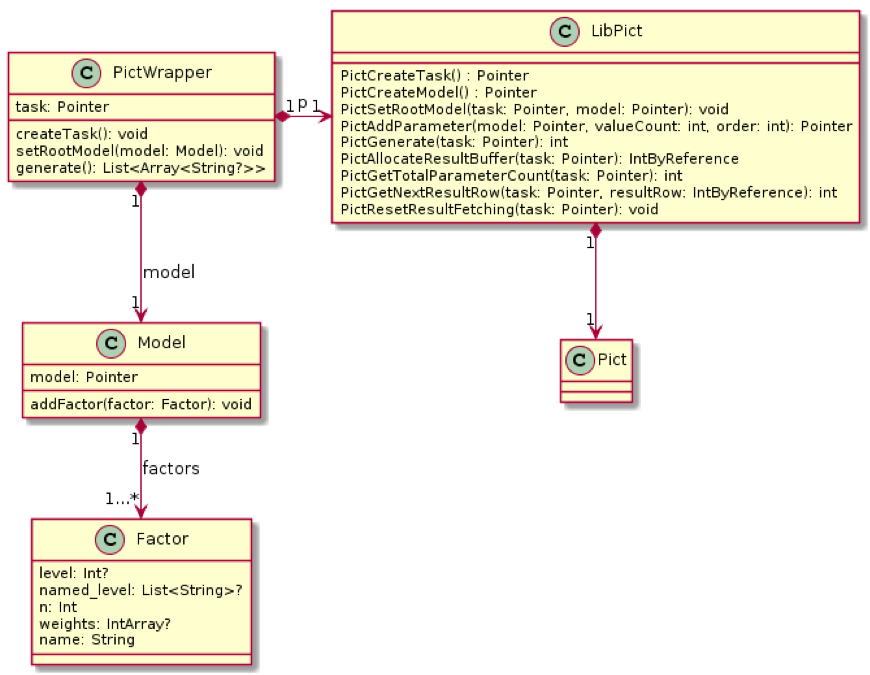
\includegraphics[keepaspectratio, width=160mm]{figs/pict4java_class}
  \caption{pict4javaのクラス図}
  \label{fig:pict4javaClass}
\end{figure}

図\ref{fig:pict4javaClass}に、pict4javaのクラス図を示す。それぞれのクラスの説明を、以下に示す。
\begin{itemize}
  \item クラスPict\\
        Microsoft社が開発したC++で記述されたPICTライブラリである。
  \item クラスLibPict\\
        JNAを用いてJavaで記述したPICTライブラリのインタフェースである。
        メソッド名は全てPICTライブラリの持つ関数名と同じである。\\
        主に使用するPICTの関数を、以下に示す。
        \begin{description}
          \item[PictAddParameter] PICTへの因子と水準の登録
          \item[PictGenerate] 組合せデータの生成
          \item[PictGetNextResultRow] 生成データの取得
        \end{description}
  \item クラスPictWrapper\\
        PICTを操作するためのクラスである。Kotlinで記述する。以下の機能を持つ。
        \begin{description}
          \item[createTask] Taskの生成と初期化をする。
                Taskは、PICTの組合せ生成処理の最小単位である。
                PICTライブラリにおけるPictCreateTaskに相当する。
          \item[setRootModel] TaskにModelの登録をする。
                Modelは因子の集合である。
                PICTライブラリにおけるPictSetRootModelに相当する。
          \item[generate] ペアワイズ法を適用した組合せの生成をする。
                PICTライブラリにおけるPictGenerateに相当する。
        \end{description}
  \item クラスModel\\
        因子の集合を保持するためのクラスである。Kotlinで記述する。
        \begin{description}
          \item[コンストラクタ] PICTライブラリにおけるModelを生成する。PictCreateModelに相当する。
          \item[addFactor] 因子(Factor)をModelに登録する。PICTライブラリにおけるPictAddParameterに相当する。
        \end{description}
  \item クラスFactor
        \begin{description}
          \item[level] 水準
          \item[named\_level] 因子の取り得る値の集合
          \item[n] 最低限組合せるペア数(デフォルトで2)
          \item[weights] 因子の取り得る値の重みの集合
          \item[name] 因子の名前
        \end{description}
        メンバ変数nの値を変えることにより、その因子については、n個の組合せを網羅する入力データを作成することができる。
\end{itemize}

\subsection{pict4javaの組込み}
\begin{figure}[tp]
  \centering
  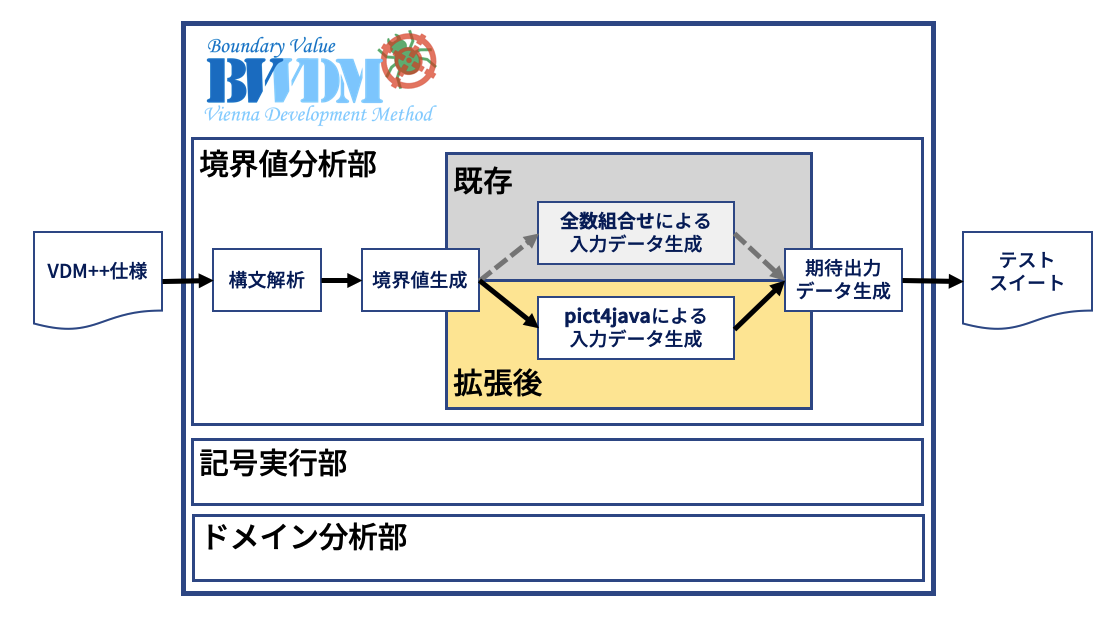
\includegraphics[keepaspectratio, width=160mm]{figs/pict4java_embed}
  \caption{pict4java組込み後の処理の流れ}
  \label{fig:pict4javaEmbed}
\end{figure}

本稿で拡張したBWDMの処理の流れを、図\ref{fig:pict4javaEmbed}に示す。
境界値分析部ではまず、テストケースの入力データとして、VDM++仕様内の引数毎における、不等式、剰余式などに合わせた境界値、及び型の最小値・最大値の境界値を、それぞれ抽出する。
既存のBWDMでは、引数毎に生成した境界値の全ての組合せを生成し、境界値テストの入力データとしていた。

拡張後のBWDMでは、全ての組合せを生成するのではなく、3.1節で作成したpict4javaを用いてペアワイズ法を適用し、入力データ生成を行う。
具体的には、境界値分析で得た因子が取り得る値をpict4javaに入力する。

境界値分析後の境界値データを受けとったpict4javaの入力データ生成アルゴリズムを、以下に示す。
また、このアルゴリズムを用いたpict4javaの処理の流れを、図\ref{fig:pict4java}に示す。

\begin{figure}[tp]
  \centering
  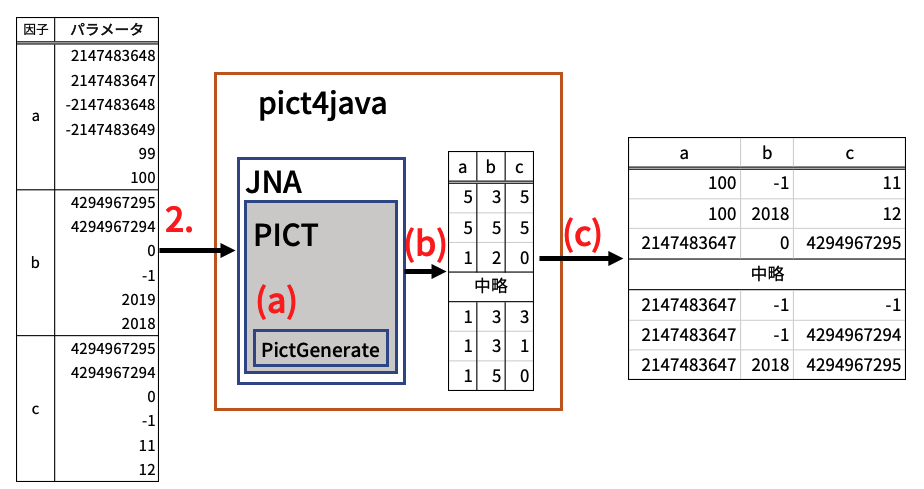
\includegraphics[keepaspectratio, width=160mm]{figs/pict4java}
  \caption{pict4javaの処理の流れ}
  \label{fig:pict4java}
\end{figure}

\begin{enumerate}
  \item 因子と、因子の取り得る値を元に、クラスFactorのインスタンスを因子の数だけ生成する。
  \item クラスModelのaddFactorメソッドを用いて、PictAddParameter関数を呼び出し、PICTに因子と因子ごとの水準を登録する。
  \item クラスPictWrapperのgenerateメソッドを用いて、ペアワイズ法を適用した組合せデータのリストを生成する。
        組合せデータは文字列型の配列のリストである。
        詳細の処理を以下に示す。
        \begin{enumerate}
          \item PictGenerate関数を用いて、PICTにペアワイズ法を適用した組合せデータを生成させる。
          \item PictGetNextResultRow関数を用いて(ア)で生成した組合せデータを1件取得する。取得したデータは、因子が取り得るパラメータ群のインデックスとなる。因子の数だけ(イ)の処理を繰り返す。
          \item (イ)で取得したデータのインデックスに該当するパラメータを用いて、組合せデータのリストを生成する。
        \end{enumerate}
  \item C)で生成したリストを、pict4javaの出力データとする。
\end{enumerate}

\section{メイン分析テストの適用による複数変数を含む条件式を含む関数のテストケース生成}
\section{対応構文の拡張}

% 適用例
\chapter{適用例}\label{cha:Indication}
\section{因子と水準の組合せ数が大きい仕様}

\begin{table}[t]
  \begin{center}
    \caption{適用結果}
    \label{tab:pict4javaTekiyourei}
    \begin{tabular}{c|c|c|c|c}
      No & \multicolumn{3}{|c|}{入力} & 期待出力                                 \\
      \hline
      \hline
      1  & 100                        & -1       & 11         & Undefined Action \\
      2  & 100                        & 2,018     & 12         & "aは100以上かつcは12以上" \\
      3  & 2,147,483,647                 & 0        & 4,294,967,295 & Undefined Action \\
      〜 & 〜                         & 〜       & 〜         & 〜 \\
      38 & 2,147,483,647                 & -1       & -1         & Undefined Action \\
      39 & 2,147,483,647                 & -1       & 4,294,967,294 & Undefined Action \\
      40 & 2,147,483,647                 & 2,018     & 4,294,967,295 & Undefined Action \\
      \hline
    \end{tabular}
  \end{center}
\end{table}

\lstset{language=}
\begin{lstlisting}[caption=因子が3、水準が(6 6 6)の関数を持つVDM++仕様。,label=fig:pict4javaSampleVdm]
class SampleClass
functions

sampleFunction : int*nat*nat -> seq of char
sampleFunction(a, b, c)==
  if(a < 100) then
    if(b > 2018) then
      "aは100未満かつbは2018より大きい"
    else
      "aは100未満かつbは2018以下"
  elseif(c < 12) then
    "aは100以上かつcは12未満"
  else
    "aは100以上かつcは12以上";

end SampleClass
\end{lstlisting}

本稿で拡張したBWDMが正しく動作することを検証するため、拡張したBWDMにVDM++仕様を適用した。
適用結果を、表\ref{tab:pict4javaTekiyourei }に示す。
適用した、因子が3、境界値分析後の水準がそれぞれ(6, 6, 6)の関数のVDM++仕様を、コード\ref{fig:pict4javaSampleVdm}に示す。

この適用例から、既存のBWDMでは216個生成していたテストケースを、拡張後のBWDMでは40個の生成に抑えており、かつ、40個のテストケースは、2個の因子のペアの組合せをすべて網羅できていることが確認できた。
すなわち、拡張したBWDMが、VDM++仕様から、ペアワイズ法を適用した境界値テストケースを正しく出力できていることが確認できた。


\section{複数変数を含む条件式を用いた仕様}
\section{class構文とoparation構文を用いた仕様}

% 考察
\chapter{考察}\label{cha:Evaluation}
\section{評価}
\subsection{膨大な数のテストケースを生成}
\lstset{language=}
\begin{lstlisting}[caption=因子が7、水準が(6 8 6 8 8 6 6)の関数を持つVDM++仕様。,label=fig:pict4javaIndication]
class ProblemClass
functions

problemFunction : nat*nat*nat*nat*nat*nat*nat -$>$ seq of char
  problemFunction(a, b, c, d, e, f, g) ==
    if(a > 4) then
      if(b mod 10 = 3) then
        if(c < 13) then
          if(b > 11) then
            "a>4 and b>11 and c<13"
          else
            if(g < 11) then
              "g<11"
            else
              "a>4 and b>10 and c<13"
        else
          if(d > 10) then
            "d>10"
          else
            if(e < 10) then
              "e<10"
            elseif(f > 10) then
              "f>10"
            else
              "a>4 and b>10 and c>=13"
      else
        "a>4 and b<=10"
    else
      "a<=4";
end ProblemClass
\end{lstlisting}

本稿で拡張したBWDMが、既存のBWDMに比べて、テストケース総数を削減できることを確認する。
膨大な数のテストケースを生成するために、因子が7、境界値分析後の水準がそれぞれ(6, 8, 6, 8, 8, 6, 6)の関数を持つVDM++仕様を、既存のBWDMと拡張後のBWDMにそれぞれ適用する。
生成結果の比較を、表2に示す。
また、適用したVDM++仕様を図5に示す。
実行環境は、macOS 10.13.6(CPU: Intel Core i5 2.3GHz, RAM: 16GB)である。
比較に用いる式を、以下に示す。

\begin{equation}
  削減率(\%) = \frac{A - B}{A} \times 100
\end{equation}

\begin{center}
  A: 既存のBWDMによって生成したテストケース総数\\
  B: 拡張したBWDMによって生成したテストケース総数\\
\end{center}

表2および式(1)より、生成テストケース数を(663552-78)/663552×100=99.98(\%)削減できた。
既存のBWDMでは、膨大な数のテストケースを生成したが、拡張後のBWDMでは、実用的な数のテストケースを生成した。
したがって、拡張後のBWDMは、境界値分析結果から生成するテストケース数が組合せ爆発を起こす可能性を排除できたと言える。
また、表2から、テストケース生成時間についても短縮できた。
以上から、拡張後のBWDMは実用性が高いと言える。

\section{拡張した\tool{}の問題点}

% おわりに
\chapter{おわりに} \label{cha:Conclusion}

%%
% 謝辞
%
\acknowledgment{}

謝辞をかくよ


%%
% 参考文献
%
\begin{thebibliography}{99}
  % 森氏の成果物
  \bibitem{ICAROB2019} Keisuke Mori, Tetsuro Katayama, Yoshihiro Kita, Hisaaki Yamaba, Kentaro Aburada, and Naonobu Okazaki: ``Development of Library Fescue Extracting Elements of Attributes and Operations of Class Diagram in UML,'' The 2019 International Conference on Artificial Life and Robotics (ICAROB2019), pp. 165--168, 2019

  \bibitem{Fescue} GitHub: ``Fescue: Feature Elements Section of Class in UML Extraction,'' https://github.com/Morichan/Fescue (最終アクセス 2019/01/25)
\end{thebibliography}

%%
% 付録
%
% \appendix{} % 付録は基本的に使わない

\end{document}
